\documentclass[border=10pt]{standalone}
\usepackage{pgfplots}
\pgfplotsset{width=7cm,compat=1.8}
\begin{document}
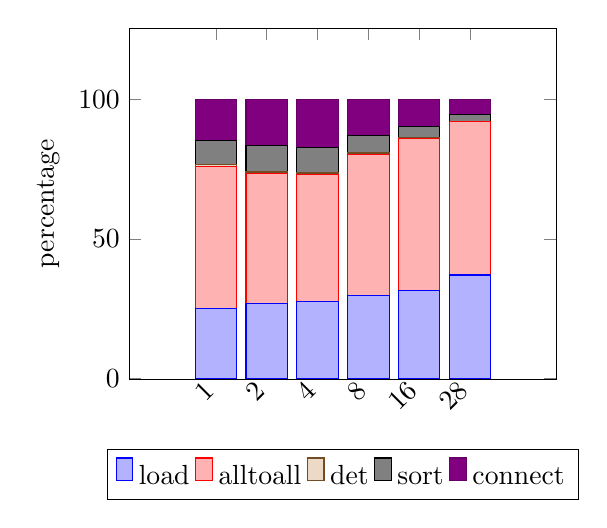
\begin{tikzpicture}
\begin{axis}[
    ybar stacked,
	bar width=15pt,
	%nodes near coords,
    enlargelimits=0.34,
    legend style={at={(0.5,-0.20)},
      anchor=north,legend columns=-1},
    ylabel={percentage},
    symbolic x coords={1, 2, 4, 8, 
		16, 28},
    xtick=data,
    x tick label style={rotate=45,anchor=east},
    ]
\addplot+[ybar] plot coordinates {(1,25.22600042) (2,26.75037249) 
  (4,27.61155984) (8,29.65530713) (16,31.66779972) (28,37.07099552)};
\addplot+[ybar] plot coordinates {(1,50.66209302) (2,46.50839332) 
  (4,45.29701305) (8,50.64404123) (16,54.18186284) (28,54.84235782)};
\addplot+[ybar] plot coordinates {(1,0.64209549) (2,0.70051676) 
  (4,0.6811092) (8,0.45425012) (16,0.30989841) (28,0.18311317)};
\addplot+[ybar] plot coordinates {(1,8.61775184) (2,9.39619732) 
  (4,9.14300033) (8,6.11830068) (16,4.1997305) (28,2.50592143)};
\addplot+[ybar] plot coordinates {(1,14.85205923) (2,16.64452011) 
  (4,17.26731758) (8,13.12810085) (16,9.64070852) (28,5.39761205)};
\legend{\strut load, \strut alltoall,\strut det,\strut sort, \strut connect}
\end{axis}
\end{tikzpicture}
\end{document}
